\documentclass{article}
\usepackage{graphicx}

\title{Axiom of Choice}
\author{Cecilia Sun}

\begin{document}

\maketitle
During the early twentieth century, the world of mathematics was roused in heated debate and controversy as mathematicians attempted to systemize and rigorize mathematics. Their goal was to construct the foundations under which past and future mathematics could be built onto. Yet, as it turns out, when we play around with the fundamental rules of our mathematical universe, we are bound to run into results that contradict our intuitive understanding of the ways in which mathematics should work. Perhaps the most famous of these controversies was the Axiom of Choice, which, when it was first conceptualized, is said to have broken mathematics. 

The modern formulation of the Axiom of Choice is as follows:

Let $(A_i)_{i\in I}$ be a collection of nonempty sets. There is a \textit{choice function} $f:A_i\to \bigcup_{i\in I}A_i$ such that for every $i\in I$, $f(A_i)$ is an element of $A_i$.

\begin{center}
    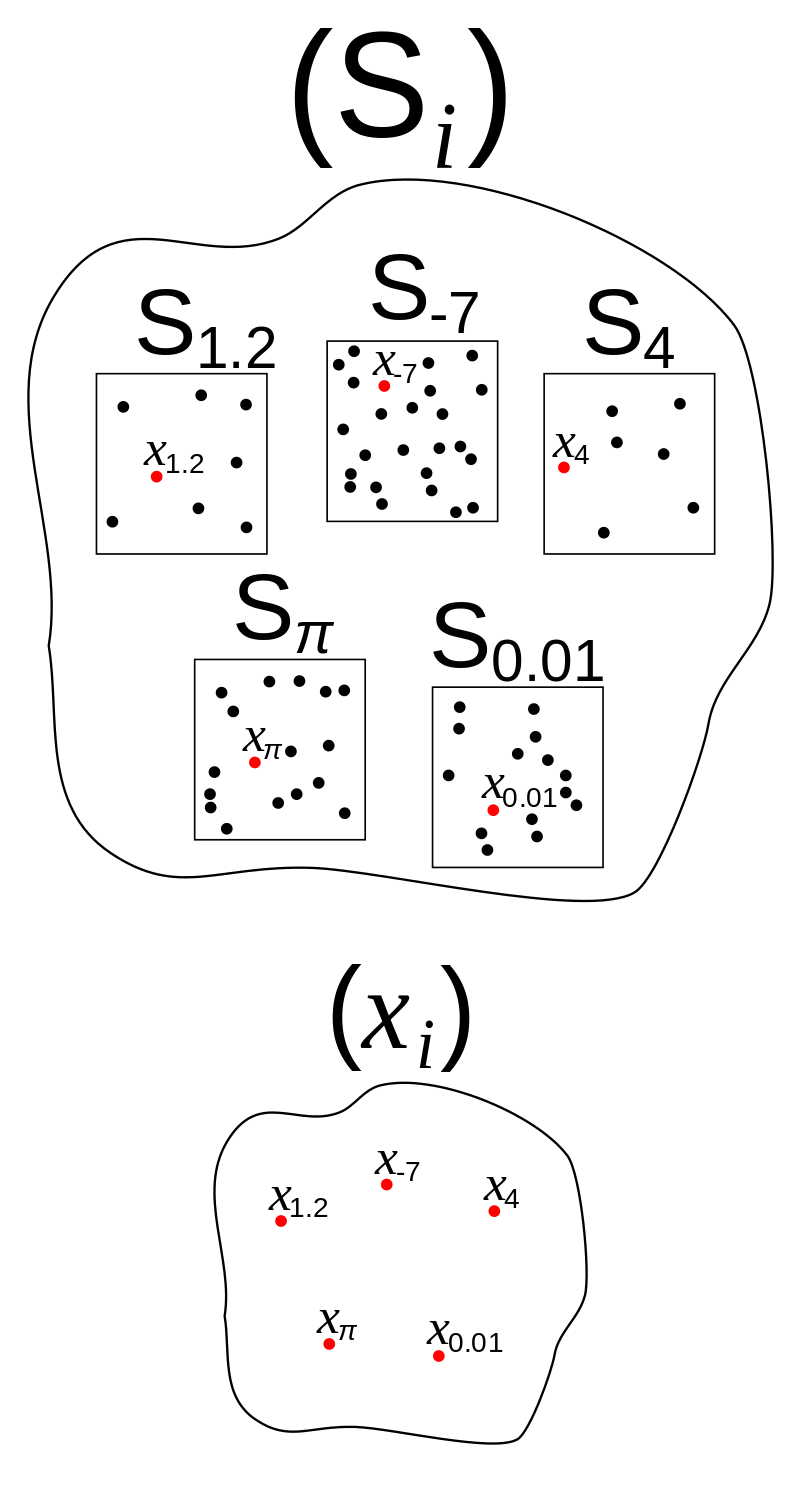
\includegraphics[scale=0.18]{images/axiom_of_choice.wikipedia.png}
\end{center}

This is a formal way of saying that there is a function that, given a bunch of sets, we can choose exactly one element from each of the sets. To understand why this seemingly innocuous axiom caused such uproar in the mathematical community, we will need to understand why it was discussed in the first place, which will require us to discuss the Well-Ordering Principle. 

We define a well order on a set to be a relation $\preceq$ that satisfies the following properties:
Irreflexivity: If a$\preceq$ b and b$\preceq$ a, then a=b.
Transitivity: If a$\preceq$b and b$\preceq$ c, then a$\preceq$ c.
Totality: Given any two elements a, b $\in$ A, either a$\preceq$ b or b$\preceq$ a.
Well-ordered: Any nonempty subset S$\subseteq$ A has a $\preceq$-minimal element.

The first three conditions define a total order – intuitively, this can be thought of as any “ordering” of things. For instance, the “less than” relation on the real numbers, or the alphabetization of strings of letters are all examples of total orders. 

The last condition makes a relation a well order – essentially, it tells us that in any subset of the set we defined our relation on, we can find an element that is “minimal”, or one that is “less than” all of the others.

However, it’s hard to find well orders on a lot of common sets! For instance, there is no least element of the open interval of reals between $0$ and $1$. 

The Well-Ordering Principle states that every set has a well order. In other words, given any set, we can always find an ordering such that every subset has a least element – even the reals! As such, mathematicians were highly skeptical of the Well-Ordering Principle when it was first formulated, even going as far to state that it was “obviously false”.

On the other hand, mathematicians had already been using the Axiom of Choice freely in their proofs. So, when, in 1904, Zermelo proved that the Axiom of Choice and the Well Ordering Principle imply each other, meaning that they were either both true or both false, the math community erupted in scandal and outrage. 

It turns out that both the Axiom of Choice and its negation both imply statements that should intuitively be true. For instance, believing in the Axiom of Choice implies that every set has a cardinality (in other words, a size), and that the countable union of countable sets is countable. However, believing in its negation implies that sets have a well-defined notion of volume, and that there is an infinite set of reals that does not contain a countably infinite set. 

Though the Axiom of Choice was initially controversial, it is nowadays accepted as an axiom by most mathematicians and is included in the standard form of axiomatic set theory, Zermelo-Fraenkel set theory with the Axiom of Choice (ZFC).
\end{document}